% Instrucciones para preparar su trabajo para la XV RPIC
% XV Reuni�n de Trabajo en Procesamiento de la Informaci�n y Control
% Autor: Comision RPIC2013
% Consultas: juanpablo.pascual@ing.unlp.edu.ar


\documentclass[a4paper,10pt]{article}
%%%%%%%%%%%%%%%%%%%%%%%%%%%%%%%%%%%%%%%%%%%%%%%%%%%%%%%%%%%%%%%%%%%%%%%%%%%%%%%%%%%%%%%%%%%%%%%%%%%%%%%%%%%%%%%%%%%%%%%%%%%%

\usepackage{rpicstyle}
\usepackage[spanish]{babel}
\usepackage{epsfig}
\usepackage{epstopdf}

%Balancear las columnas
\usepackage{balance}

%Use PostScript Times Roman as the default font instead of Computer Times Roman.
\usepackage{times}

\affiliation{
\dag Club Atl\'{e}tico Rosario Central, Rosario, Santa Fe, Argentina. \\
{\ negro@canallas.com} \\
\ddag Club Atl\'{e}tico River Plate, Ciudad Aut\'{o}noma de Buenos Aires, Argentina. \\
{\ caloi@gallinas.com.ar}
}

\begin{document}
\title{Multifractal classification of bread crumb digital images}
\author{Rodrigo Baravalle$^{\dag }$ y Carlos Loiseau$^{\ddag }$}
\maketitle

\renewcommand{\refname}{REFERENCIAS}

\balance

%\resumen
% For english written papers use \abstract
\abstract
Adequate models of the bread crumb structure can be critical for understanding flow and transport
processes in bread, creating synthetic bread crumb images for photo-realistic rendering, evaluating similarities and establishing quality features of different bread crumbs types.

In this article multifractal analysis, employing the multifractal spectrum (MFS), has been applied to study the structure of the bread crumb in four varieties of breads ({\em baguette}, {\em sliced}, {\em bran}, and {\em sandwich}). The extracted dimensions can be used to discriminate among bread crumbs from different types. Also, high correlations were found between some of these parameters and the porosity, coarseness, and heterogeneity of the samples. These results demonstrate that the MFS is an appropriate tool for characterizing the internal structure of the bread crumb and thus may be used to establish important quality properties it should have.

The MFS has shown to provide local and global image features that are both robust and low-dimensional, leading to features vectors that capture essential information for classification tasks. Based on this, in this work we also apply the MFS for bread crumb classification of slices of different bread types. Results show that the MFS based classification is able to distinguish different bread crumbs with very high accuracy. The multifractal modeling of the bread crumb structure can be an appropriate method for parameterizing and simulating the appearance of different bread crumbs.
%Estas instrucciones se presentan para ayudar a los autores a preparar su trabajo en el formato definitivo correspondiente a la XV Reuni\'{o}n de
%Trabajo en Procesamiento de la Informaci\'{o}n y Control. El resumen no debe exceder las 200 palabras.
\endresumen
% For english written papers use \endabstract

\palabras
% For english written papers use \keywords
Por favor, incluya hasta cinco palabras clave que identifiquen en forma concreta su trabajo.
\endpalabras
% For english written papers use \endkeywords

\section{INTRODUCCI\'{O}N}
One of the most important factors of the quality of a bread loaf is related to its crumb structure. Close examination of different slices reveals considerable variation in the cell size even within a single sample of the same bread type. 

Fractals methods could be appropriate to characterize this structure. Fractal and multifractal analysis of images have proved to capture useful properties of the underlying material being represented. These features have been successfully applied in different areas, such as medicine \cite{Andjelkovic2008,Yu2011} and texture classification \cite{Wendt2009}. In food research, fractal and multifractal analysis has been applied in the study of apple tissues \cite{Mendoza2010}, pork sirloins \cite{Serrano2012} and others \cite{Quevedo2002}. Through several procedures \cite{Peitgen2004, Gonzales2008}, it is possible to obtain different Fractal Dimensions (FD), each of them capturing a different property of the material ({\em e.g.}, porosity, rugosity).

For each material, the results obtained in classification tasks and in the data analysis in the feature extraction process are useful in quality measurements of real samples and also in the validation of synthetic representations of them. In other words, these processes are useful to determine if a given image presents the observed features in that material, allowing to associate quality measure parameters to it. In~\cite{Fan2006}, a quality bread crumb test based on Gabor filters was performed in that paper, obtaining good results. Nevertheless, a small database was used ($30$ images). In \cite{Gonzales2008} several fractal features were obtained for one type of bread, demonstrating that a vector of FDs would be capable of obtaining key features of its crumb texture more accurately than using a single FD.

In this work we propose the application of the Multifractal Spectrum (MFS) \cite{Xu2006} to describe and classify among different bread types. One of the main features of the MFS is its bi-Lipschitz invariance, which includes perspective transforms (viewpoint changes) and smooth texture surface deformations. It is shown that the MFS is also locally invariant to affine changes in illumination. These features are useful to describe bread crumb structures in a robust way that results adequate for the purposes of this study.

The proposed method is compared to other classifiers that uses state-of-the-art features for texture classification. The results of this feature extraction procedure show that the classifier is robust and presents good discrimination properties to distinguish between different bread types and also bread from non bread images. The objectives of this study were: (1) to evaluate if the MFS can be applied to characterize and discriminate the bread crumb structure from different bread types from digital images, and (2) to investigate the efectiveness of the method in the classification of these structures.

This paper is organized as follows. In section 2 the theory underlying fractal sets is introduced, and the materials and methods employed in this work are presented. In section 3 the results obtained in the characterization and classification procedures are shown and discussed. In section 4 the conclusions are summarized, as well as possible future works.


%Se solicita a los autores que sigan cuidadosamente estas instrucciones para la preparaci\'{o}n de sus trabajos. Este documento es en s\'{\i} mismo un ejemplo del formato que deber\'{\i}a tener el art\'{\i}culo final que se publicar\'{a} en los anales de la Reuni\'{o}n.

%Los manuscritos deben ser escritos en Espa\~{n}ol o en Ingl\'{e}s y no deben sobrepasar el l\'{\i}mite m\'{a}ximo de 6 (seis) p\'{a}ginas, de tama\~{n}o A4.

\section{DESARROLLO}

\subsection{Instrucciones generales}
%Los trabajos deben estar escritos en formato a doble columna, balanceadas en la \'ultima p\'agina, en un cuadro de 165 mm $\times $ 245 mm. El ancho de las columnas debe ser de 80 mm con 5 mm de distancia entre columnas. Los autores deben enviar los manuscritos \'{u}nicamente en versi\'{o}n electr\'{o}nica, en formato PDF. Los trabajos se recibir\'{a}n en su versi\'{o}n final, no se aceptar\'{a}n res\'{u}menes de trabajos.

\subsubsection{Importante}
%Las p\'{a}ginas no deben numerarse. Verifique que el archivo enviado no est\'{e} protegido.

\subsection{Tama\~{n}o de fuentes y espaciado}
%Los trabajos deben estar escritos con espaciado simple. El espaciado puede incrementarse solamente en caso de ser necesario por el uso de sub\'{\i}ndices o super\'{\i}ndices. El tama\~{n}o de las fuentes usadas en el texto de las ilustraciones debe ser, como m\'{\i}nimo, de 2 mm.
%El tama\~{n}o de fuentes para el cuerpo del texto debe ser de 10 puntos (1 punto = 0.35 mm).

\subsection{Ilustraciones}
%Todas las ilustraciones deben ser originales. Deben ubicarse a lo largo de todo el trabajo, y no agrupadas al final. Los ep\'{i}grafes de las figuras deben ubicarse debajo de las mismas, como se muestra en la Fig. \ref{clementeypereyra}.

%\begin{figure}[ht]
%  \centering{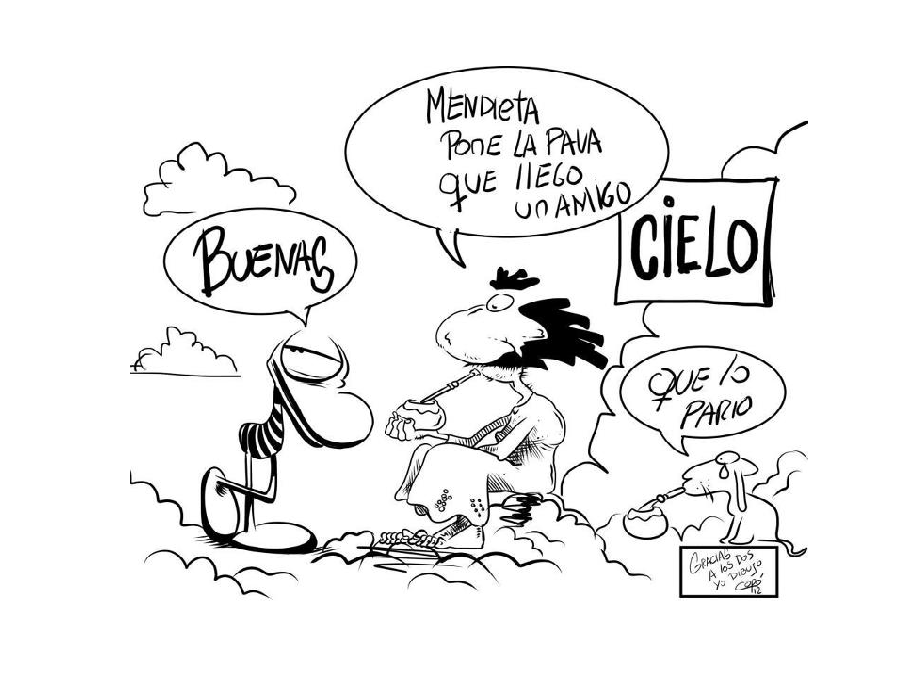
\epsfig{file=clementeypereyra.eps, width=0.8\columnwidth}}
%  \caption{Clemente e Inodoro Pereyra, homenaje a sus creadores.}\label{clementeypereyra}
%\end{figure}

Los t\'{\i}tulos de las Tablas deben ser breves, y deben ubicarse sobre la tabla correspondiente, como se muestra en la Tabla \ref{posiciones}. Utilice los ambientes tabla y tabla* provistos en rpictyle.sty, si el idioma es el espa\~nol.

\begin{tabla}[b]
  \caption{Posiciones Primera B Nacional 2011/12.}\label{posiciones}
  \vspace{2mm}
  \centering
  \begin{tabular}{|c|l|c|} \hline
  Pos. & Equipo & Puntos\\ \hline\hline
  $1�$ & River Plate & 73 \\ \hline
  $2�$ & Quilmes & 72\\ \hline
  $3�$ & Instituto & 70\\ \hline
  $4�$ & Rosario Central & 69\\ \hline
  $\vdots$ & $\vdots$ & $\vdots$ \\ \hline
  $20�$ & Chacarita Juniors & 32\\ \hline
  \end{tabular}
\end{tabla}

Las ecuaciones, las figuras y las tablas deben numerarse con numeraci\'{o}n ar\'{a}biga.

El n\'{u}mero de las ecuaciones debe estar alineado junto al margen derecho

\begin{equation}
\dot{x}=f_{1}\left( x_{1},t\right) +\alpha x_{2}\sin \left( \theta \right),
\label{eq1}
\end{equation}
mientras que la ecuaci\'{o}n debe ubicarse centrada con respecto a la columna.

Las palabras ``Figura'' y ``Ecuaci\'{o}n'' deben abreviarse, usando ``Fig.'' y ``Ec.'' cuando se usen en medio de una oraci\'{o}n. Sin embargo, deben
escribirse en forma completa cuando se empleen al comienzo de la oraci\'{o}n. Cuando se haga referencia a una ecuaci\'{o}n el n\'{u}mero de la misma debe estar entre par\'{e}ntesis y se recomienda evitar utilizar Ec. en los casos en que sea posible. Por ejemplo: ``...de (\ref{eq1}) resulta...''.

\subsection{Formato de las Referencias}
En el cuerpo del trabajo, las referencias deben citarse por n\'{u}meros entre corchetes. En el siguiente p\'{a}rrafo se presenta un ejemplo.

En Rosario dicen, para contrarrestar tanto aburrimiento, que tienen las minas m\'{a}s lindas del pa\'{i}s: parece un invento de la misma \'{i}ndole que la fama que los petisos y los pelados se hicieron de s\'{i} mismos, para compensar por abajo lo que la naturaleza les priv\'{o} de arriba. Yo supongo que esta fama, entonces, es un invento de las rosarinas, para reparar el abandono que padecen los domingos cuando todos los rosarinos, sea por Central o por \~{N}uls, todos se van al f\'{u}tbol \cite{Caloi_2006}. Fontanarrosa adhiere totalmente a este culto. Muestras de esto son muchas de sus obras \cite{Negro_2000,Negro2_2000} o aquellos memorables chistes futboleros como ``Es tan pobre la situaci\'{o}n actual del f\'{u}tbol argentino, que el pr\'{o}ximo cuadrangular amistoso lo vamos a hacer entre tres equipos'' \cite{Negro_1990}.

La lista de referencias debe escribirse en orden de aparici\'{o}n, siguiendo el estilo general que se muestra en el ejemplo m\'{a}s abajo, correspondiente al provisto por el estilo IEEEtran.bst.

\section{CONCLUSIONES}
Es importante que los autores sigan estas ``reglas'' para que los anales puedan elaborarse r\'{a}pida y eficientemente.

% La secci�n REFERENCIAS puede realizarse mediante BibTeX, usando
%\bibliographystyle{IEEEtran}
%\bibliography{rpicbib}

% IEEEtran.bst puede descargarse en: http://www.ctan.org/tex-archive/macros/latex/contrib/IEEEtran/bibtex

% o manualmente

\begin{thebibliography}{1}

\bibitem{Caloi_2006}
C.~Loiseau, ``Homenaje a fontanarrosa,'' in \emph{Proceedings from Senado de la
  Naci\'{o}n}, Buenos Aires, Argentina, 2006, pp. 165--172.

\bibitem{Negro_2000}
R.~Fontanarrosa, \emph{No te vayas, campe\'{o}n}.\hskip 1em plus 0.5em minus
  0.4em\relax Buenos Aires, Argentina: Editorial {S}udamericana {S}. {A}.,
  2000.

\bibitem{Negro2_2000}
R.~Fontanarrosa, \emph{Puro f\'{u}tbol}.\hskip 1em plus 0.5em minus 0.4em\relax Buenos
  Aires, Argentina: Ediciones de la {F}lor, 2000.

\bibitem{Negro_1990}
R.~Fontanarrosa, ``El f\'{u}tbol es sagrado,'' \emph{Recopilaciones de chistes sueltos},
  vol. 148, no.~18, pp. 35--48, 1990.

\bibitem{ej_1}
A.B.~Autor1, {\em T\'{i}tulo del libro}. Lugar de edici\'{o}n: Editorial, a\~{n}o.

\bibitem{ej_2}
A.B.~Autor1, C.D.~Autor2 y E.~Autor3, ``T\'{i}tulo del art\'{i}culo,'' {\em T\'{i}tulo de la revista en cursiva}, volumen, n\'{u}mero, p\'{a}ginas, a\~{n}o.

\bibitem{ej_3}
A.B.~Autor1 y C.D.~Autor2, ``T\'{i}tulo del art\'{i}culo,'' {\em T\'{i}tulo del congreso en cursiva}, Lugar, a\~{n}o, p\'{a}ginas.

\end{thebibliography}

\end{document} 
